\subsubsection{Fahrradbox}
Fahrradboxen bieten im Gegensatz zu einem Fahrradständer eine sichere Verwahrung des Fahrrades. Zusätzlich können andere Gegenstände wie die Jacke oder der Helm verstaut werden. Falls es sich um eine zweistöckige Fahrradbox handelt, führt dies zu einer geringen Nutzerfreundlichkeit, denn das Heben des Fahrrades ist nicht für alle Personen möglich. Zusätzlich benötigt eine Fahrradbox viel Platz.

\begin{figure}[H]
    \centering
    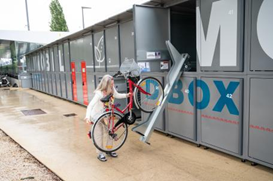
\includegraphics[width=0.5\textwidth]{images/fahrradbox.png}
    \caption{Fahrradboxen in Vorarlberg \citev{fahrradbox}}
    \label{fig:fahrradbox}
\end{figure}
